%=====================================================================
% 4  矩阵积分
% 原文：Section 4. Matrix integrals（arXiv:2409.03117v1, p. 51--62）
%=====================================================================
\section{矩阵积分}

\begin{keytakeaways}
\begin{itemize}
  \item \textbf{物理图像：}矩阵积分把随机矩阵的谱理论与二维曲面的组合拓扑统一起来。对大 $N$，配分函数对数关于耦合常数的展开按胖图（即带边曲面）的亏格分层，每一项都携带因子 $N^{2-2{\rm g}}$，而 $2-2{\rm g}$ 正是亏格 ${\rm g}$ 的闭曲面的欧拉示性数。
  \item \textbf{数学工具：}Feynman 定理加张量缩并：把每个 $i$-价花加胖，再沿匹配保向粘合，缩并给出 $\widetilde{\Bbb F}(\sigma)=N^{\nu(\widetilde\Gamma_\sigma)}$，即边界分支数 $\nu$ 成为 $N$ 的幂次；再由欧拉公式 $b=2{\rm g}-2+\nu$ 与标度变换 $\hbar\mapsto\hbar/N$ 即得亏格展开。
  \item \textbf{关键结论：}'t Hooft 定理：极限 $W_\infty=\lim_{N\to\infty}N^{-2}\log\widehat Z_N$ 由亏格零的平面胖图支配；而 $\log\widehat Z_N/N^2$ 按 $N^{-2{\rm g}}$ 的展开，其第 ${\rm g}$ 阶恰由亏格 ${\rm g}$ 的连通曲面贡献。实对称矩阵情形允许带子扭转 $180^\circ$ 的粘合，此时亏格可取半整数。
  \item \textbf{易错点：}作用量中 $\Tr(A^m)$ 的系数是 $1/m$ 而非 $1/m!$；Wigner 半圆律的第 $2m$ 阶矩等于 Catalan 数 $C_m$；Hermite 多项式按权 $e^{-x^2}$（而非 $e^{-x^2/2}$）正交，其范数平方为 $2^nn!\sqrt{\pi}$。
\end{itemize}
\end{keytakeaways}

\bigskip
\noindent\rule{\textwidth}{0.6pt}
\bigskip

设 ${\frak h}_N$ 为 $N$ 阶 Hermitian 矩阵所成空间。${\frak h}_N$ 上的内积由 $B(A_1,A_2)=\Tr(A_1A_2)$ 给出。本节考虑如下形式的积分：
$$
Z_N:=\hbar^{-\frac{N^2}{2}}\int_{{\frak h}_N}e^{-\frac{S(A)}{\hbar}}dA,
$$
其中 Lebesgue 测度 $dA$ 按条件
$$
\int_{{\frak h}_N} e^{-\frac{{\rm Tr}(A^2)}{2}}dA=1
$$ 
归一化（这样就不必处处携带 $\sqrt{2\pi}$ 因子），而
$$
S(A):=\frac{\Tr(A^2)}{2}-\sum_{m\ge 1} g_m\frac{\Tr(A^m)}{m}
$$
是作用量泛函。\footnote{注意这里除以 $m$ 而不是 $m!$。下文将说明这种归一化为何更为方便。} 我们关心的是 $Z_N$ 关于 $g_i$ 的展开系数在大 $N$ 时的行为。对这一行为的研究将引导我们不去考虑简单的 Feynman 图，而是考虑胖图（或带状图）——它们实际上是二维曲面。因此，在进一步推进之前，我们需要做一些二维组合拓扑。
% [Tutor Note: 原文脚注强调作用量里除以 m 而非 m!，这一点决定了全部组合因子。由 B_m=(m-1)!\Tr(A^m) 以及 Feynman 定理，每个 i 价花给出 (i-1)! 而非 i!；而 log Z_N 的展开式中已带 1/i^{n_i}n_i!，再对每个花的循环次序 S_{i-1} 求和给出 (i-1)! 倍，二者相抵后分母只剩 i^{n_i}n_i!。核对顶点系数时切勿再补一个 1/i!；这也是后文把 \prod_i i!^{n_i} 换成 \prod_i i^{n_i} 的来源。]

\subsection{胖图}
回想 Feynman 定理的证明：给定有限个花（flower）以及在其各边端点所成集合 $T$ 上的一个匹配 $\sigma$，把落在同一对中的点连接（粘合）起来，便得到图 $\Gamma_\sigma$。

现在，给定一个 $i$-价花，把它内接于一个闭圆盘 $D$（使各边的端点都落在边界上），再在 $D$ 中取它的一小块管状邻域。这样就得到一个边界分段光滑的区域。我们为该区域及其边界取标准定向，并称之为一个\emph{胖 i-价花}。一个胖 $i$-价花的边界形如 $P_1Q_1P_2Q_2 \ldots P_iQ_iP_1$，其中 $P_i,Q_i$ 为角点，区间 $P_jQ_j$ 是 $\partial D$ 上的弧，而 $Q_jP_{j+1}$ 是位于 $D$ 内部的（光滑）弧（见图~\ref{fig:10}）。

\begin{figure}[htbp]
  \centering
  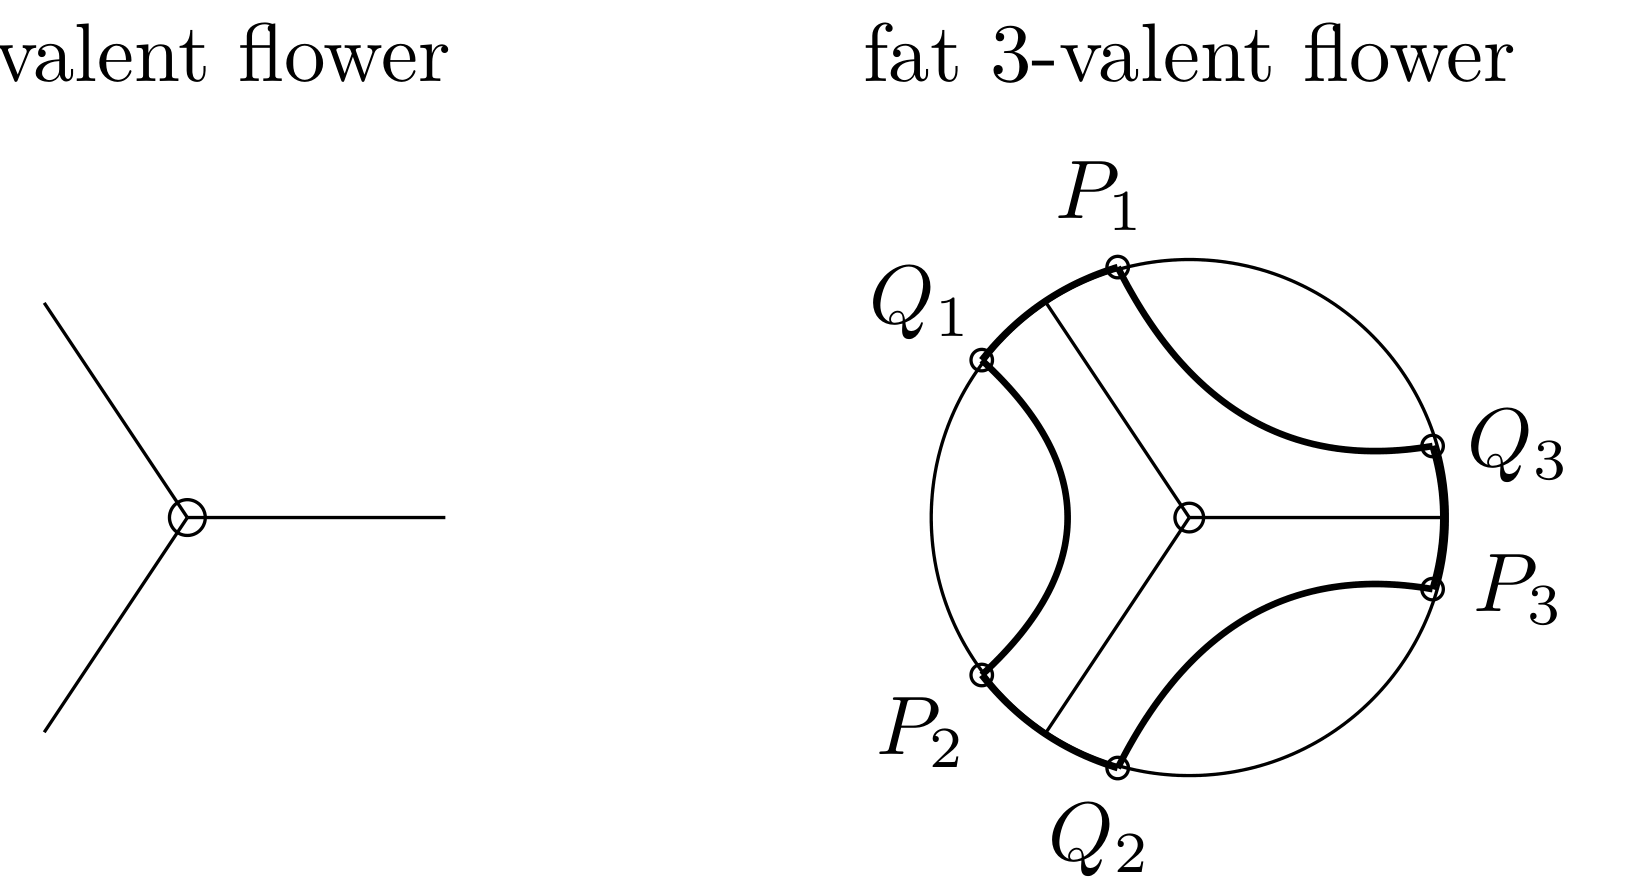
\includegraphics[width=6.92cm]{figures/fig-10.png}
  \caption{（原文无图题）\figorig{52}{10}}
  \label{fig:10}
\end{figure}


现在，给定一族通常的花以及如上所述的一个匹配 $\sigma$，我们取相应的胖花，并按 $\sigma$ 沿区间 $P_jQ_j$ 保向地粘合它们。这将产生一个带边的紧定向曲面（其边界由区间 $Q_{j}P_{j+1}$ 粘合而成）。我们用 $\widetilde \Gamma_{\sigma}$ 记这个曲面，并称之为 $\Gamma$ 关于 $\sigma$ 的\emph{加胖}。图的加胖称为\emph{胖图}（或\emph{带状图}）。

因此，胖图并不只是一个带边的定向曲面，而是这样的曲面连同把它分割成胖花的一个划分。

注意同一个图 $\Gamma$ 可以有许多互不同胚（尽管同伦等价）的加胖，特别地，加胖的亏格 ${\rm g}$ 并\emph{不}由 $\Gamma$ 决定（见图~\ref{fig:11}）。

\begin{figure}[htbp]
  \centering
  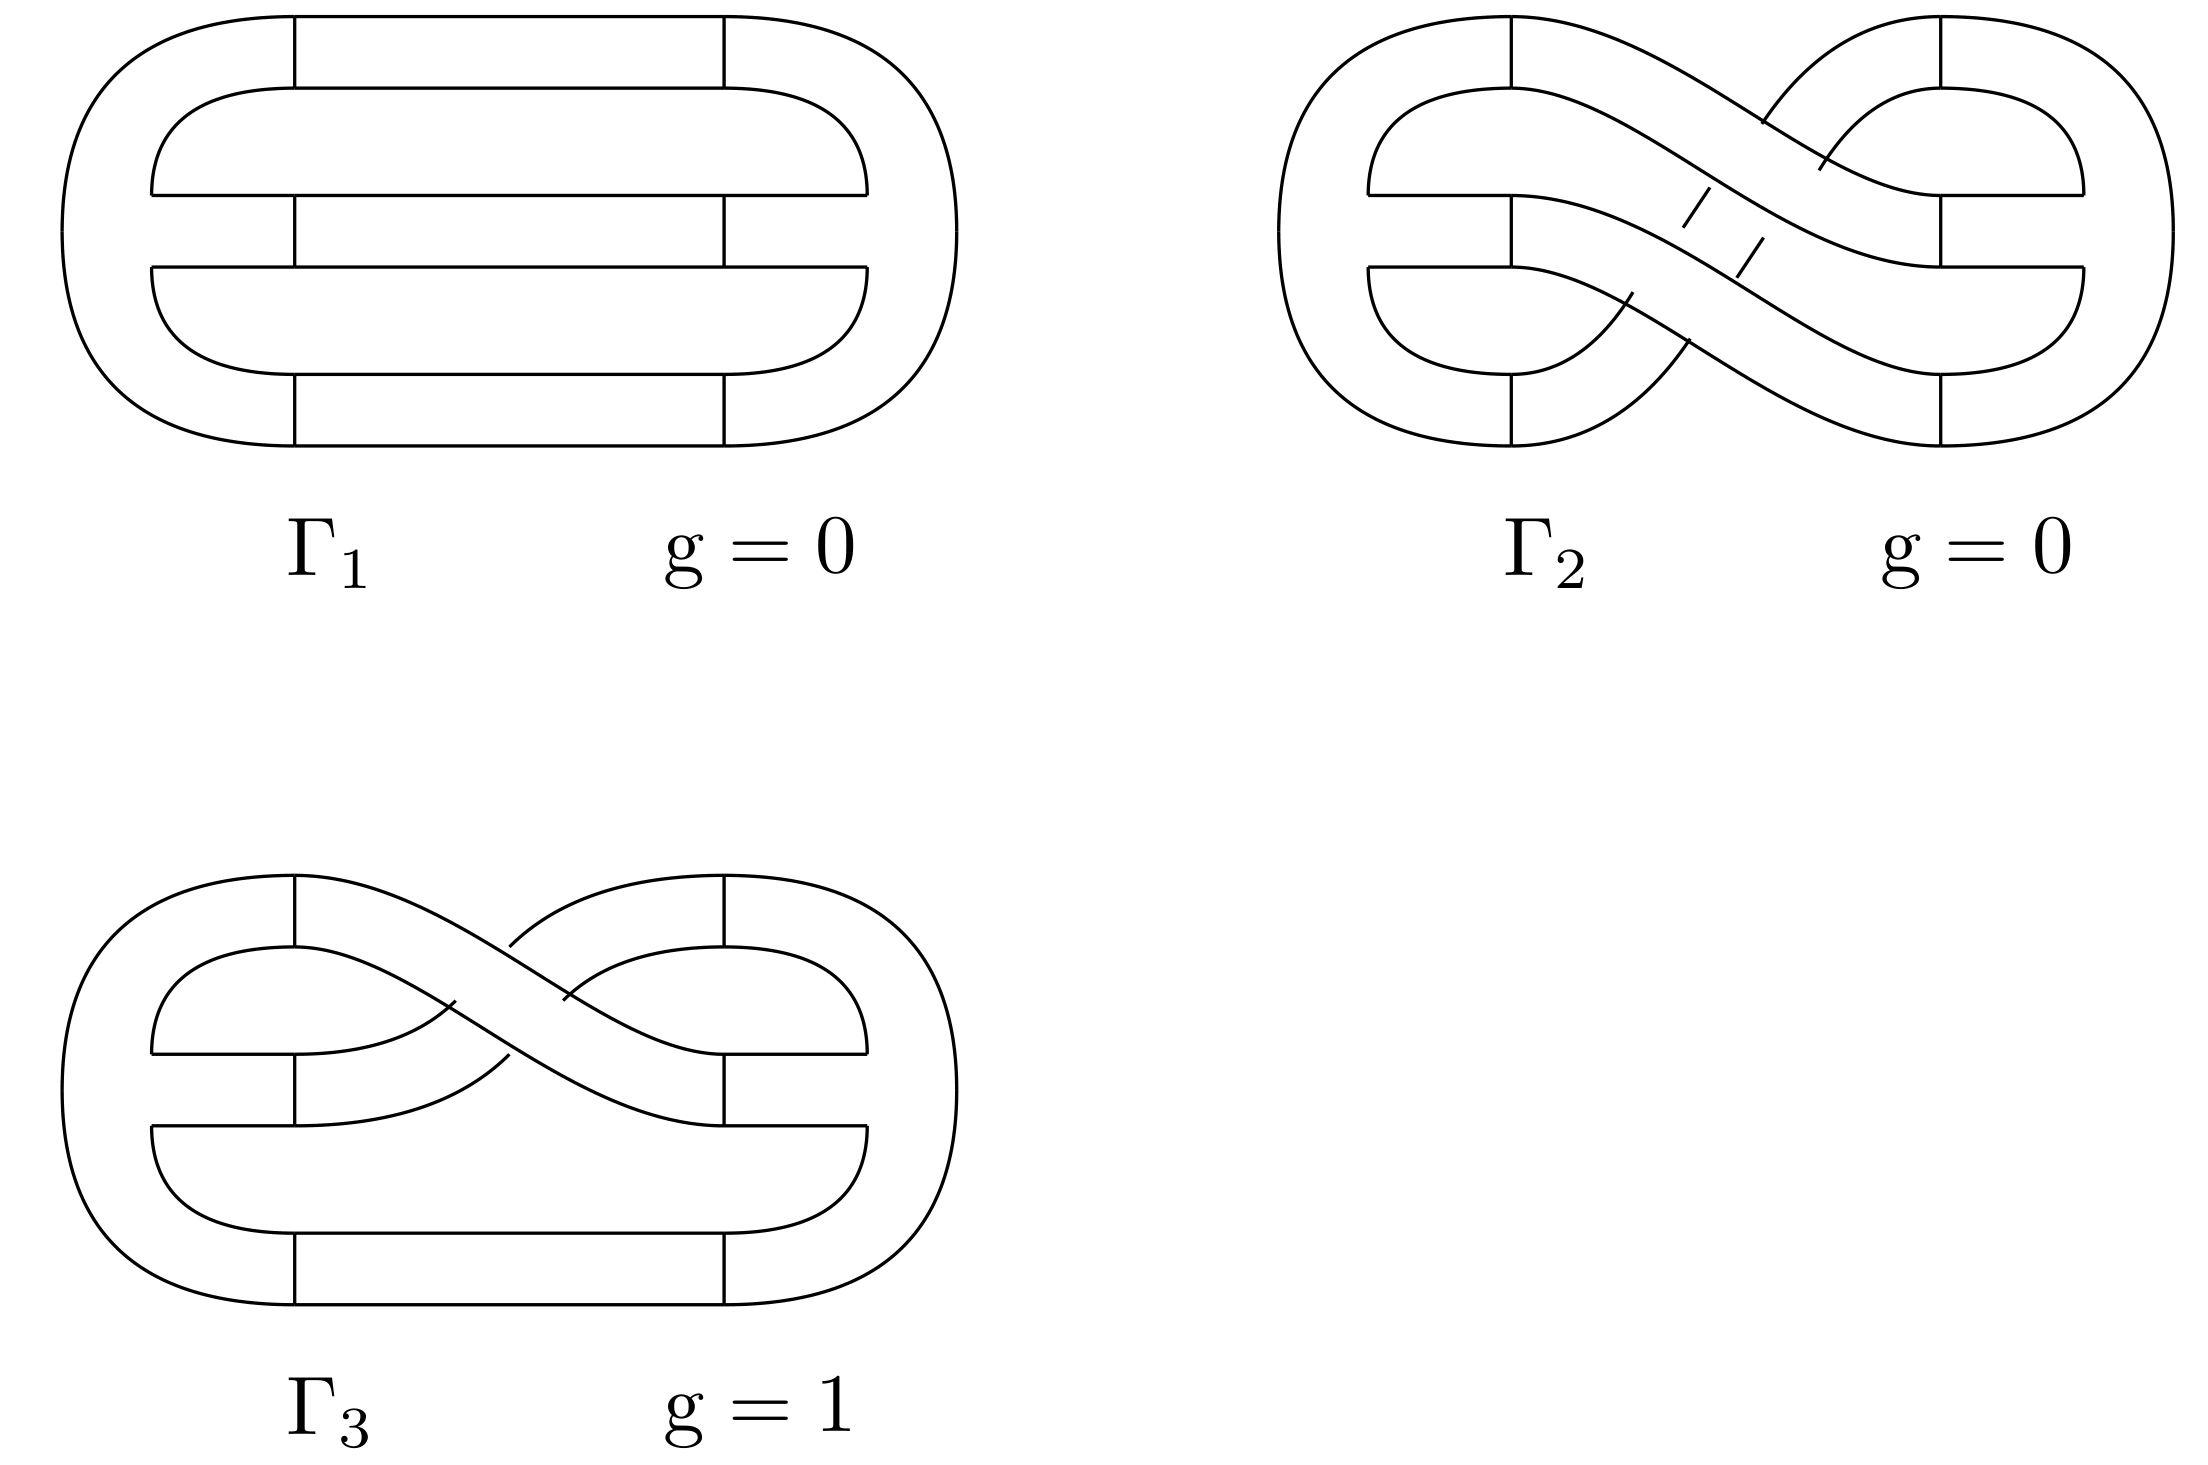
\includegraphics[width=9.35cm]{figures/fig-11.png}
  \caption{由胖花粘合胖图\figorig{52}{11}}
  \label{fig:11}
\end{figure}

\subsection{大 $N$ 极限中的矩阵积分、平面图与亏格展开}

现在回到积分 $Z_N$ 的研究。我们有
$$
B_m(A,...,A)=(m-1)!\Tr(A^m).
$$ 
于是由 Feynman 定理，
$$
\log Z_N=\sum_{\bold n}\prod_i \frac{(g_i\hbar^{\frac{i}{2}-1})^{n_i}}{i!^{n_i}n_i!}
\sum_{\sigma\in \Pi_c(T_{\bold n})}\Bbb F(\sigma),
$$
其中求和遍历集合 $\Pi_c(T_{\bold n})$——即 $T=T_{\bold n}$ 的所有使图 $\Gamma_\sigma$ 连通的匹配，而 $\Bbb F(\sigma)$ 表示用 $\sigma$ 对张量 $(m-1)!\Tr(A^m)$ 作缩并的结果。下面来计算 $\Bbb F(\sigma)$。

设 $\lbrace e_i\rbrace$ 是 $\Bbb C^N$ 的标准基，$\lbrace e_i^*\rbrace$ 是对偶空间中的对偶基。则张量 $\Tr(A^m)$ 可以写成
$$
\Tr(A^m)=\sum_{i_1, \ldots ,i_m=1}^N
(e_{i_1}\otimes e_{i_2}^*\otimes e_{i_2}\otimes e_{i_3}^*\otimes \cdots
\otimes e_{i_m}\otimes e_{i_1}^*,A^{\otimes m}).
$$
因此
$$
B_m=\sum_{s\in S_{m-1}}\sum_{i_1, \ldots ,i_m=1}^N
s(e_{i_1}\otimes e_{i_2}^*\otimes e_{i_2}\otimes e_{i_3}^*\otimes \cdots
\otimes e_{i_m}\otimes e_{i_1}^*)
$$
（对 $m$-价花各边的所有可能的循环次序求和）。于是
$$
\Bbb F(\sigma)=\sum_{s\in \prod_i S_{i-1}^{n_i}} \widetilde {\Bbb F}(s\sigma),
$$
其中 $\widetilde {\Bbb F}(\sigma)$ 是按胖图 $\widetilde\Gamma_{\sigma}$ 缩并张量
\begin{equation}\label{tenso}
\sum_{i_1,...,i_m=1}^Ne_{i_1}\otimes e_{i_2}^*\otimes e_{i_2}\otimes e_{i_3}^*\otimes \cdots
\otimes e_{i_m}\otimes e_{i_1}^*
\end{equation} 
所得的结果。由此可得
$$
\log Z_N=
\sum_{\bold n}\prod_i \frac{g_i^{n_i}\hbar^{n_i(\frac{i}{2}-1)}}{i!^{n_i}n_i!}
\sum_{\sigma\in \Pi(T_{\bold n})}\sum_{s\in \prod_i S_{i-1}^{n_i}}\widetilde {\Bbb F}(s\sigma)=
$$
$$
\sum_{\bold n}\prod_i \frac{g_i^{n_i}\hbar^{n_i(\frac{i}{2}-1)}}{i^{n_i}n_i!}
\sum_{\sigma}\widetilde {\Bbb F}(\sigma)
$$
（分母中的 $\prod_i i!^{n_i}$ 被换成了 $\prod_i i^{n_i}$，因为在和 $\sum_{s,\sigma}\widetilde {\Bbb F}(s\sigma)$ 中，每一项 $\widetilde {\Bbb F}(\sigma)$ 都出现 $|\prod_i S_{i-1}^{n_i}|=\prod_i (i-1)!^{n_i}$ 次）。

对带边曲面 $\Sigma$，用 $\nu(\Sigma)$ 表示其边界连通分支的个数。

\begin{proposition}\label{fatt}
$\widetilde {\Bbb F}(\sigma)=N^{\nu(\widetilde\Gamma_{\sigma})}$.
\end{proposition}

\begin{proof}
可以把和 \eqref{tenso} 中的每一项看成用 $i_1,i_2,i_2,i_3, \ldots ,i_m,i_1$ 对胖 $m$-价花边界上的角点 $P_1,Q_1, \ldots ,P_m,Q_m$ 所作的一种标号。现在，用 $\sigma$ 对某一组这样的单项式作缩并，其结果非零当且仅当下标沿着 $\widetilde\Gamma_{\sigma}$ 的每个边界分支都是常数（见图 12）。由此即得结论。
\end{proof}

\begin{figure}[htbp]
  \centering
  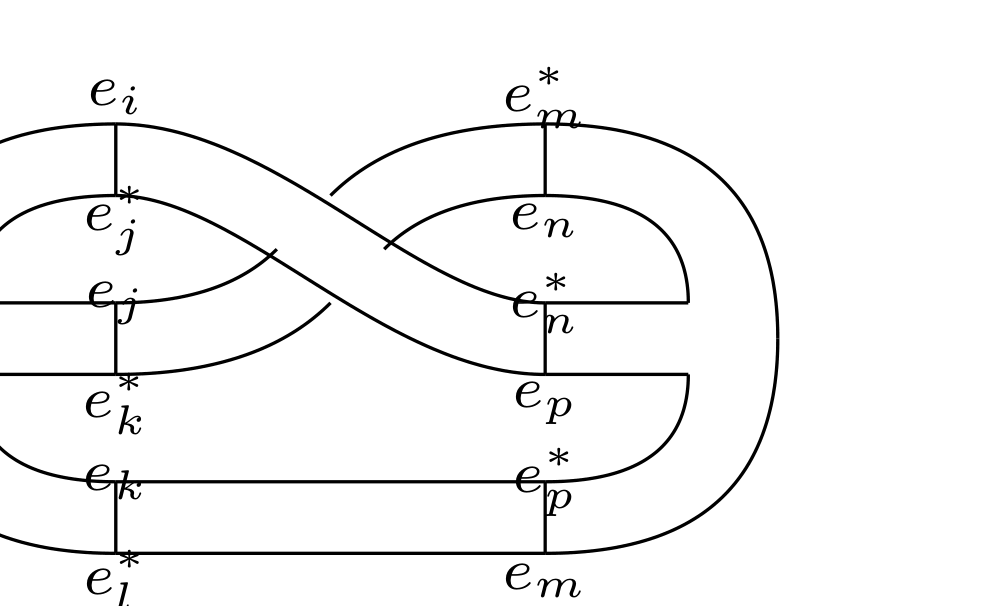
\includegraphics[width=4.2cm]{figures/fig-12.png}
  \caption{由胖图定义的缩并。\figorig{54}{12}}
  \label{fig:12}
\end{figure}

设 $\widetilde G_c(\bold n)$ 是连通胖图的同构类所成集合，其中对每个 $i\ge 1$ 恰有 $n_i$ 个 $i$-价顶点。对 $\widetilde\Gamma\in \widetilde G_c(\bold n)$，用 $b(\widetilde\Gamma)$ 表示其底层的通常图 $\Gamma$ 的边数减去顶点数。

\begin{corollary}\label{fatt1}
$$
\log Z_N=\sum_{\bold n}\prod_i (g_i\hbar^{\frac{i}{2}-1})^{n_i}
\sum_{\widetilde\Gamma\in \widetilde G_c(\bold n)}\frac{N^{\nu(\widetilde\Gamma)}}
{|{\rm Aut}(\widetilde\Gamma)|}=
$$
$$
\sum_{\bold n}\prod_i g_i^{n_i}
\sum_{\widetilde\Gamma\in \widetilde G_c(\bold n)}\frac{N^{\nu(\widetilde\Gamma)}\hbar^{b(\widetilde\Gamma)}}
{|{\rm Aut}(\widetilde\Gamma)|}.
$$
\end{corollary}

\begin{proof} 
令 $\Bbb G_{\bold n}^{\rm cyc}:=
\prod_i (S_{n_i}\ltimes (\Bbb Z/i\Bbb Z)^{n_i})$。
此群作用在 $T_{\bold n}$ 上，使得对任意 $g\in \Bbb G_{\bold n}^{\rm cyc}$ 都有
$\widetilde\Gamma_{\sigma}=\widetilde\Gamma_{g\sigma}$。
此外，该群在给出同一个胖图 $\widetilde\Gamma_{\sigma}$ 的所有 $\sigma$ 之集上可迁地作用，并且任一 $\sigma$ 的稳定子恰为
${\rm Aut}(\widetilde\Gamma_{\sigma})$。由此即得结论，因为 $|\Bbb G_{\bold n}^{\rm cyc}|=\prod_i i^{n_i}n_i!$ 
正好消去各分母。
\end{proof}
% [Tutor Note: 对称因子 |Aut(\widetilde\Gamma)| 此处是“保胖花结构的图自同构”，不是底层的普通图自同构：它包含每个花上循环次序的旋转（(Z/iZ)^{n_i}）。群 \Bbb G_{\bold n}^{\rm cyc} 的阶 \prod_i i^{n_i}n_i! 与 Feynman 展开的分母相消，剩下 1/|Aut|，这正是 Burnside 式的计数；用组合方法直接数胖图时容易把旋转对称漏掉或因重复计数而多除，务必核对。]

现在，对任意带边的紧连通曲面 $\Sigma$，用 ${\rm g}(\Sigma)$ 表示 $\Sigma$ 的亏格。则对连通胖图
$\widetilde\Gamma$，
$$
b(\widetilde\Gamma)=
2{\rm g}(\widetilde\Gamma)-2+\nu(\widetilde\Gamma)
$$ 
（即负的欧拉示性数）。于是若定义
$$
\widehat Z_N(\hbar):=Z_N(\tfrac{\hbar}{N}),
$$
便得到
% [Tutor Note: 从推论 4.2 到定理 4.3 的关键一步是把 \hbar 标度为 \hbar/N 并用 \nu-b=2-2g。明细如下：推论中每项为 g_i^{n_i}N^{\nu}\hbar^{b}，把 \hbar 换成 \hbar/N 得到 N^{\nu-b}\hbar^{b}；又由欧拉公式 b=2g-2+\nu 得 \nu-b=2-2g。于是 N 的幂次只剩 2-2g，而 \hbar 的幂次 b 恰好等于 \prod_i(i/2-1)n_i=\frac12\sum i n_i-\sum n_i（后者用了边数 E=\frac12\sum i n_i）。核对任意给定图的 N 幂次时，先数边界分支 \nu 与 b=E-V，再算 \nu-b 最稳妥。实对称（扭转）情形公式形式不变，但 g=1-\chi/2 可取半整数（RP^2：\chi=1 故 g=1/2；Klein 瓶：\chi=0 故 g=1），于是 N^{-2g} 展开中出现 N^{-1},N^{-3},... 奇次幂，与可定向情形的纯偶次幂不同；根源在于扭转粘合使曲面可以非定向。]

\begin{theorem}\label{lnZ}
$$
\log\widehat Z_N=
\sum_{\bold n}\prod_i (g_i\hbar^{\frac{i}{2}-1})^{n_i}
\sum_{\widetilde\Gamma\in \widetilde G_c(\bold n)}
\frac{N^{2-2{\rm g}(\widetilde\Gamma)}
}{|{\rm Aut}(\widetilde\Gamma)|}.
$$
\end{theorem}

这蕴含着下述重要结果，它属于 't Hooft。

\begin{theorem} \label{tHooft} (1) 存在极限 
$W_\infty:=\lim_{N\to \infty}\frac{\log\widehat Z_N}{N^2}$。该极限由下述公式给出：
$$
W_\infty=
\sum_{\bold n}\prod_i (g_i\hbar^{\frac{i}{2}-1})^{n_i}
\sum_{\widetilde\Gamma\in \widetilde G_c(\bold n)[0]}
\frac{1}{|{\rm Aut}(\widetilde\Gamma)|},
$$
其中 $\widetilde G_c(\bold n)[0]$ 表示\textbf{平面}连通胖图之集，即亏格为零者。

(2) 此外，存在展开
$$
\frac{\log\widehat Z_N}{N^2}=\sum_{{\rm g}\in \Bbb Z_{\ge  0}}a_{\rm g}N^{-2\rm g},
$$
其中
$$
a_{\rm g}=\sum_{\bold n}\prod_i (g_i\hbar^{\frac{i}{2}-1})^{n_i}
\sum_{\widetilde\Gamma\in \widetilde G_c(\bold n)[{\rm g}]}
\frac{1}{|{\rm Aut}(\widetilde\Gamma)|},
$$
而
$\widetilde G_c(\bold n)[{\rm g}]$ 表示亏格为 ${\rm g}$ 的连通胖图之集。
\end{theorem}

\begin{remark} 亏格为零的胖图之所以称为平面的，是因为其底层的通常图可以无自交地放在二维球面（从而也放在平面）上。
\end{remark}

\begin{remark} 't Hooft 定理可以用通常的 Feynman 图展开来解释。具体地说，它表明对大的 $N$，$\log Z_N(\frac{\hbar}{N})$ 的首项贡献来自 Feynman 图展开中对应于平面图（即可以嵌入二维球面的图）的那些项。
\end{remark} 

\subsection{实对称矩阵上的积分}

也可以考虑在 $N$ 阶实对称矩阵所成空间 ${\frak s}_N$ 上的矩阵积分。即令
$$
Z_N=\hbar^{-\frac{N(N+1)}{4}}\int_{{\frak s}_N} e^{-\frac{S(A)}{\hbar}}dA,
$$ 
其中 $S$ 与 $dA$ 同上。下面把定理 \ref{tHooft} 推广到这一情形。

如前，大 $N$ 极限的考虑引导我们考虑胖花及其粘合。然而，粘合的确切方式现在有所不同。也就是说，在 Hermitian 情形我们有
$(e_i\otimes e_j^*,e_k\otimes e_l^*)=
\delta_{il}\delta_{jk}$，这迫使我们保向地粘合胖花。另一方面，
在实对称情形 $e_i^*=e_i$，而泛函
$e_i\otimes e_j$ 在对称矩阵空间上的内积由
$(e_i\otimes e_j,e_k\otimes e_l)=
\delta_{ik}\delta_{jl}+\delta_{il}\delta_{jk}$ 给出。
这意味着，除了通常的（保向）粘合胖花之外，现在还必须允许把带子扭转 $180^\circ$ 后再粘合。这样得到的胖图称为\emph{扭转胖图}。也就是说，扭转胖图是一个带边曲面（可能不可定向），连同把它分割成胖花的一个划分，以及每个胖花上的定向（这些定向在切口处可以一致，也可以不一致，见图 13）。

\begin{figure}[htbp]
  \centering
  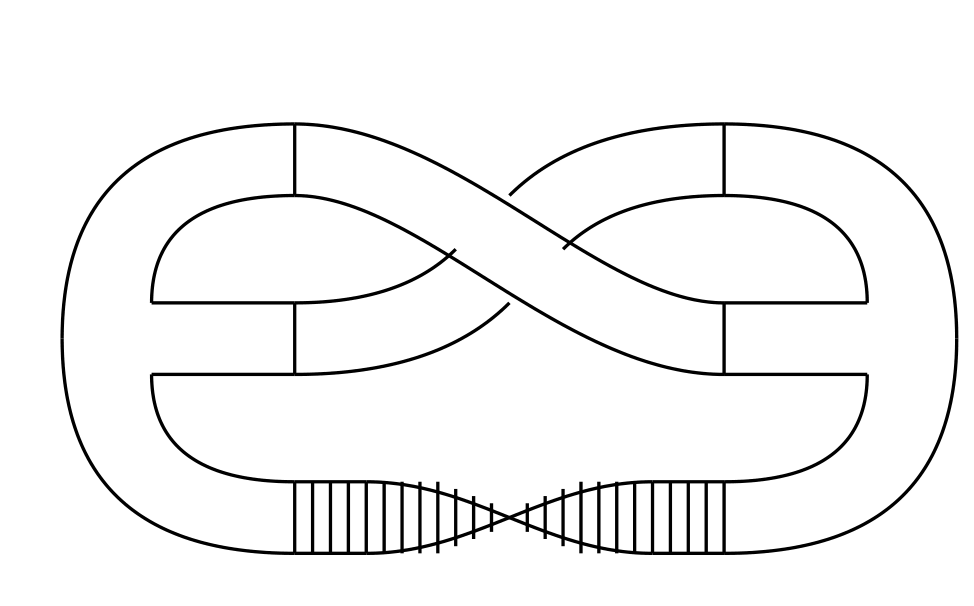
\includegraphics[width=4.12cm]{figures/fig-13.png}
  \caption{扭转胖图\figorig{56}{13}}
  \label{fig:13}
\end{figure}
 

现在，与 Hermitian 情形类似可以证明，$\log \widehat Z_N$ 的 $\frac{1}{N}$ 展开
（其中 $\widehat Z_N:=Z_N(\frac{2\hbar}{N}))$）由与前面相同的公式给出，只是求和改为遍历扭转胖图之集 $\widetilde G_c^{\rm tw}(\bold n)$：

\begin{theorem}\label{lnZ1}
$$
\log\widehat Z_N=
\sum_{\bold n}\prod_i (g_i\hbar^{\frac{i}{2}-1})^{n_i}
\sum_{\widetilde\Gamma\in \widetilde G_c^{\rm tw}(\bold n)}
\frac{N^{2-2{\rm g}(\widetilde\Gamma)}
}{|{\rm Aut}(\widetilde\Gamma)|}.
$$
\end{theorem}

这里，（可能不可定向的）曲面的亏格 ${\rm g}$ 对闭曲面用
${\rm g}:=1-\frac{\chi}{2}$ 定义，其中 $\chi$ 是欧拉示性数。于是 $\Bbb R\Bbb P^2$ 的亏格为 $\frac{1}{2}$，Klein 瓶的亏格为 $1$，如此等等。

特别地，我们有下述 't Hooft 定理的类比。

\begin{theorem} \label{tHooft1} (1) 存在极限 
$W_\infty:=\lim_{N\to \infty}\frac{\log\widehat Z_N}{N^2}$。该极限由下述公式给出：
$$
W_\infty=
\sum_{\bold n}\prod_i (g_i\hbar^{\frac{i}{2}-1})^{n_i}
\sum_{\widetilde\Gamma\in \widetilde G_c^{\rm tw}(\bold n)[0]}
\frac{1}{|{\rm Aut}(\widetilde\Gamma)|},
$$
其中 $\widetilde G_c^{\rm tw}(\bold n)[0]$ 表示\textbf{平面}连通扭转胖图之集，即亏格为零者。

(2) 此外，存在展开
$$
\frac{\log\widehat Z_N}{N^2}=\sum_{{\rm g}\in \frac{1}{2}\Bbb Z_{\ge 0}}a_{\rm g}N^{-2\rm g},
$$
其中
$$
a_{\rm g}=\sum_{\bold n}\prod_i (g_i\hbar^{\frac{i}{2}-1})^{n_i}
\sum_{\widetilde\Gamma\in \widetilde G_c^{\rm tw}(\bold n)[{\rm g}]}
\frac{1}{|{\rm Aut}(\widetilde\Gamma)|},
$$
而
$\widetilde G_c^{\rm tw}(\bold n)[{\rm g}]$ 表示亏格为 ${\rm g}$ 的连通扭转胖图之集。
\end{theorem}

\begin{exercise} 考虑在 $N$ 阶四元数 Hermitian 矩阵所成空间 ${\frak q}_N$ 上的矩阵积分。证明：此时结果与实情形相同，只是每个扭转胖图都带一个符号 $(-1)^\nu$，其中 $\nu$ 是边界分支的个数。换言之，$\log Z_N^{\rm quat}(\hbar)$ 等于把 $N$ 换成 $-N$ 后的 $\log Z_{2N}^{\rm real}(\hbar)$。

\textbf{提示：} 利用四元数酉群 $U(N,\Bbb H)$ 是 $Sp(2N)$ 的实形式，而 ${\frak q}_N$ 是表示 $\Lambda^2V$ 的实形式，其中 $V$ 是 $Sp(2N)$ 的标准（向量）表示。与实对称矩阵情形比较：那里相关的表示是 $O(N)$ 的 $S^2V$；而复数 Hermitian 矩阵情形则是 $GL(N)$ 的 $V\otimes V^*$。
\end{exercise} 

\subsection{由多边形粘合曲面的方式数与 Wigner 半圆律}

矩阵积分内容如此丰富，以至于最平凡的例子也会归结为一个不平凡的计数问题。具体地说，取复 Hermitian 矩阵上的矩阵积分 $Z_N$，令 $\hbar=1$ 并取
$S(A)=\frac{\Tr(A^2)}{2}-s\frac{\Tr(A^{2m})}{2m}$，其中 $s^2=0$
（即我们在环 $\Bbb C[s]/(s^2)$ 上工作）。则由定理 \ref{tHooft} 得到
$$
\int_{{\frak h}_N}\Tr(A^{2m})e^{-\frac{\Tr(A^2)}{2}}dA
=P_m(N),
$$
其中 $P_m(N)$ 是由公式
$$
P_m(N)=\sum_{{\rm g}\ge 0}\varepsilon_{\rm g}(m)N^{m+1-2\rm g},
$$ 
给出的多项式，而 $\varepsilon_{\rm g}(m)$ 是用一个有标号边的 $2m$ 边形粘合出亏格为 ${\rm g}$ 的曲面的方式数，即把各边配对、再把相配的边彼此保向地粘合起来的方式数。事实上，此时只有一个 $2m$ 价的胖花，它必须与自身粘合；因此直接应用我们的 Feynman 规则就归结为统计由多边形粘合出给定亏格曲面的方式数。

这个积分的值由下述不平凡的定理给出。

\begin{theorem} (Harer-Zagier, \cite{HZ} 1986) \label{howmany}
$$
P_m(x)=\frac{(2m)!}{2^mm!}\sum_{p=0}^m\begin{pmatrix}m\\ p\end{pmatrix}
2^p\frac{x(x-1) \ldots (x-p)}{(p+1)!}.
$$
\end{theorem}

该定理将在后面几个小节中证明。

考察 $P_m$ 的首项系数，即得

\begin{corollary}\label{Catalan}
用一个 $2m$ 边形粘合出球面的方式数，是 Catalan 数 $C_m=\frac{(2m)!}{m!(m+1)!}=\frac{1}{m+1}\binom{2m}{m}$。
\end{corollary}

推论 \ref{Catalan} 其实还有另一个（初等组合的）证明，如下所示。对 $2m$ 边形的边集上的每个匹配 $\sigma$，用直线段连接相配各边的中点（图 14）。从几何上看显然：若这些线段互不相交，则粘合给出球面。我们断言其逆亦真。事实上，设不然，即对循环排序的边 $a,b,c,d$，边 $a$ 与 $c$ 相连、$b$ 与 $d$ 相连。那么容易看出，把这两对边粘合起来会给出一个带孔的环面（$m=2$ 时则不带孔）。但带孔的（开）环面不能嵌入球面（例如它包含 $K_5$ 的一个拷贝），矛盾。

\begin{figure}[htbp]
  \centering
  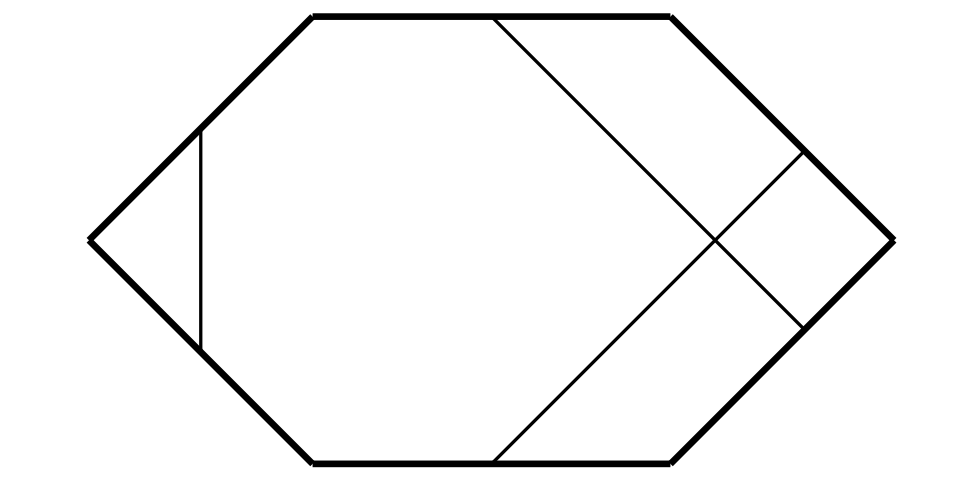
\includegraphics[width=4.04cm]{figures/fig-14.png}
  \caption{一个 $6$ 边形的边配对。\figorig{58}{14}}
  \label{fig:14}
\end{figure}

现在只剩下统计用互不相交的线段连接各边中点的方式数。假设我们画出这样一条线段，使其左侧有 $2k$ 条边、右侧有 $2l$ 条边（于是 $k+l=m-1$）。那么我们就面临把这两组各 $2k$ 与 $2l$ 条边用互不相交的线连接起来的问题。这表明粘合方式数 $D_m$ 满足递推
$$
D_m=\sum_{k+l=m-1}D_kD_l,\ D_0=1.
$$
换言之，生成函数
$$
h(x):=\sum_m D_mx^m=1+x+ \cdots
$$ 
满足方程 $h(x)-1=xh(x)^2$。由此得到
$$
h(x)=\frac{1-\sqrt{1-4x}}{2x},
$$ 
从而 $D_m=C_m$。证毕。

推论 \ref{Catalan} 可用来推出随机矩阵理论中的下述基本结果，它由 Wigner 于 1955 年发现。

\begin{theorem} (Wigner 半圆律)
设 $f$ 是 $\Bbb R$ 上在无穷远处至多多项式增长的连续函数。则
$$
\lim_{N\to \infty} \frac{1}{N}\int_{{\frak h}_N}{\rm }{\rm Tr} f(\tfrac{A}{\sqrt{N}})e^{-\frac{{\rm Tr}(A^2)}{2}}=
\frac{1}{2\pi}\int_{-2}^2f(x)\sqrt{4-x^2}dx.
$$
\end{theorem}

该定理之所以称为半圆律，是因为它说：按“高斯酉系综”（即密度为 $e^{-\frac{\Tr(A^2)}{2}}dA$）分布的大型随机 Hermitian 矩阵，其本征值密度的图形是半圆。特别地，我们看到对大的 $N$，$A$ 的几乎所有本征值都落在区间 $[-2\sqrt{N},2\sqrt{N}]$ 内，因此该极限与 $f$ 在 $[-2,2]$ 之外的值无关。
% [Tutor Note: 半圆律的矩方法：定理断言对任意多项式 f 有极限，而由 Catalan 数只验证了 f(x)=x^{2m} 的情形。半圆分布 \frac{1}{2\pi}\sqrt{4-x^2}dx 的 2m 阶矩正是 C_m（奇数阶矩为 0），例如 m=1 时 \frac{1}{2\pi}\int_{-2}^2 x^2\sqrt{4-x^2}dx=1。做替换 x=2\cos\theta 可化为 Beta 积分 \frac{2^{2m}}{\pi}\int_0^\pi\cos^{2m}\theta\sin^2\theta\,d\theta，其值为 \frac{(2m)!}{m!(m+1)!}。注意定理左边的归一化：f=1 时两边都等于 1，故文中 1/N 而非常见的 1/N^{m+1} 是正确的。]

\begin{proof} 
由 Weierstrass 关于闭区间上连续函数可被多项式一致逼近的定理，可以假定
$f$ 是多项式（习题：请论证这一步）。于是只需在
$f(x)=x^{2m}$ 时验证结论。此时由推论 \ref{Catalan}，左端等于 $C_m$。另一方面，初等计算给出
$$
\frac{1}{2\pi}\int_{-2}^2x^{2m}\sqrt{4-x^2}dx=C_m,
$$ 
由此即得定理。
\end{proof}

\subsection{Hermite 多项式}

下面给出的定理 \ref{howmany} 的证明\footnote{这个证明取自 D. Jackson 的讲义。}要用到 Hermite 多项式。因此先回顾它们的性质。

Hermite 多项式由公式
$$
H_n(x)=(-1)^ne^{x^2}\frac{d^n}{dx^n}e^{-x^2}.
$$
定义。于是 $H_n(x)$ 的首项为 $(2x)^n$。

我们在下述定理中汇集 $H_n(x)$ 的标准性质。
% [Tutor Note: 归一化约定在此务必留意：这里取权函数 e^{-x^2}（物理学家约定 H_n），因此 \frac{1}{\sqrt{\pi}}\int e^{-x^2}H_mH_n dx=2^nn!\delta_{mn}；若改用概率论约定 He_n（权 e^{-x^2/2}，即 ∫e^{-x^2/2}He_mHe_n=\sqrt{2\pi}n!\delta_{mn}），则定理 (iii)(iv)(v) 的所有常数都要改。另注意 (ii) 中 H_n(x)e^{-x^2/2} 是 L=-\frac12\partial^2+\frac12x^2 的本征函数，本征值 n+\frac12：权 e^{-x^2}=(e^{-x^2/2})^2 恰好来自把 L 的本征函数除以 e^{-x^2/2} 后去掉 Gaussian 因子，这一“权 = 波函数模方”的关系是正交性的来源。]

\begin{theorem} \label{Hermite}
(i) $H_n(x)$ 的指数生成函数为
$$
f(x,t)=\sum_{n\ge 0}H_n(x)\frac{t^n}{n!}
=e^{2xt-t^2}.
$$ 

(ii) $H_n(x)$ 满足微分方程
$f''-2xf'+2nf=0$。换言之，
$H_n(x)e^{-x^2/2}$ 是算子 $L=-\frac{1}{2}\partial^2+\frac{1}{2}x^2$（量子谐振子的哈密顿量）的本征函数，本征值为 $n+\frac{1}{2}$。

(iii) $H_n(x)$ 彼此正交：
$$
\frac{1}{\sqrt{\pi}}\int_{-\infty}^{\infty}e^{-x^2}H_m(x)H_n(x)dx=
2^nn!\delta_{mn}.
$$
此外，函数 $H_n(x)e^{-\frac{x^2}{2}}$ 构成 $L^2(\Bbb R)$ 的一组正交基。  

(iv) 有
$$
\frac{1}{\sqrt{\pi}}\int_{-\infty}^{\infty}e^{-x^2}x^{2m}H_{2k}(x)dx=
\frac{(2m)!}{(m-k)!}2^{2(k-m)}
$$
（若 $k>m$，答案为零）。

(v) 有
$$
\frac{H_r^2(x)}{2^rr!}=\sum_{k=0}^r\frac{r!}{2^kk!^2(r-k)!}H_{2k}(x).
$$
\end{theorem}
 
\begin{proof}（略证）
(i) 由算子 $\sum_{n\ge 0} (-1)^n\frac{t^n}{n!}\frac{d^n}{dx^n}$ 
把函数 $g(x)$ 映为 $g(x-t)$ 这一事实立得。

(ii) 由 (i) 以及函数 $f(x,t)$ 满足偏微分方程
$$
f_{xx}-2xf_x+2tf_t=0.
$$ 
即得。

(iii) 正交性可由 (i) 直接积分得到：
$$
\frac{1}{\sqrt{\pi}}\int_{\Bbb R}f(x,t)f(x,u)e^{-x^2}dx=\frac{1}{\sqrt{\pi}}\int_{\Bbb R}e^{2ut-(x-u-t)^2}dx=e^{2ut}.
$$ 
于是函数 $H_n(x)e^{-\frac{x^2}{2}}$ 在 $L^2(\Bbb R)$ 中构成正交系。

为说明这些函数是完备的，用 $E\subset L^2(\Bbb R)$ 记它们的张成 $\Bbb C[x]e^{-\frac{x^2}{2}}$ 的闭包。用 Taylor 多项式逼近函数 $e^{ipx}$，容易看出对任意 $p\in \Bbb R$ 都有 $e^{ipx-\frac{x^2}{2}}\in E$。
于是对任意紧支光滑函数 $\phi\in C_0^\infty(\Bbb R)$ 有
$$
\phi(x)e^{-\frac{x^2}{2}}=\int_{\Bbb R} \widehat \phi(p)e^{ipx-\frac{x^2}{2}}dp\in E.
$$
其中 $\widehat \phi$ 是 $\phi$ 的（适当归一化的）Fourier 变换。换言之，$C_0^\infty(\Bbb R)$ 在 $E$ 中稠密。
但 $C_0^\infty(\Bbb R)$ 显然在 $L^2(\Bbb R)$ 中稠密，故 $E=L^2(\Bbb R)$，如所断言。

(iv) 由 (i)，应计算
$\int_{\Bbb R}x^{2m}e^{2xt-t^2}e^{-x^2}dx$。
该积分等于
$$
\int_{\Bbb R}x^{2m}e^{-(x-t)^2}dx=\int_{\Bbb R}(y+t)^{2m}e^{-y^2}dy=
=\sqrt{\pi}
\sum_p \begin{pmatrix} 2m\\ 2p\end{pmatrix} \frac{(2m-2p)!}{2^{m-p}(m-p)!}t^{2p}.
$$
现在逐个提取系数即得结果。

(v) 由 (iii)，只需证明
$$
\frac{1}{\sqrt{\pi}}\int_{\Bbb R}H_r^2(x)H_{2k}(x)
e^{-x^2}dx=\frac{2^{r+k}r!^2(2k)!}{k!^2(r-k)!}
$$
为证此恒等式，把三个生成函数之积积分。由 (i) 有
$$
\frac{1}{\sqrt{\pi}}\int_{\Bbb R}f(x,t)f(x,u)f(x,v)e^{-x^2}dx=
$$
$$
\frac{1}{\sqrt{\pi}}\int_{\Bbb R}e^{2(ut+uv+tv)-(x-u-t-v)^2}dx
=e^{2(ut+tv+uv)}.
$$
提取 $t^ru^rv^{2k}$ 的系数即得结果。
\end{proof}

\subsection{定理 \ref{howmany} 的证明}
我们需要计算积分
$$
\int_{{\frak h}_N}\Tr(A^{2m})e^{-\frac{\Tr(A^2)}{2}}dA.
$$
为此注意被积函数在酉矩阵共轭下不变。因此该积分可以化为对 $A$ 的本征值 $\lambda_1, \ldots ,\lambda_N$ 的积分。

更确切地说，考虑谱映射 $\sigma: {\frak h}_N\to \Bbb R^N/S_N$。
众所周知（H. Weyl），直像
$\sigma_*dA$ 由公式
$\sigma_*dA=Ce^{-\sum_i\frac{\lambda_i^2}{2}}\prod_{i<j} (\lambda_i-\lambda_j)^2d\lambda$ 
给出，其中 $C>0$ 是一个与本文无关的归一化常数。于是有
$$
P_m(N)=\frac{NJ_m}{J_0},\ J_m:=\int_{\Bbb R^N}(\frac{1}{N}\sum_i\lambda_i^{2m})
e^{-\sum_i \frac{\lambda_i^2}{2}}\prod_{i<j} (\lambda_i-\lambda_j)^2d\lambda.
$$
为计算 $J_m$，我们将使用 Hermite 多项式。注意 $H_n(x)$ 是首项系数为 $2^n$ 的 $n$ 次多项式，故有
$$
\prod_{i<j}(\lambda_i-\lambda_j)= 2^{-\frac{N(N-1)}{2}}
\det (H_k(\lambda_\ell)),
$$ 
其中 $k$ 遍历集合
$0,1, \ldots ,N-1$，而 $\ell$ 遍历 $1,...,N$。于是得到
\begin{equation}
\begin{gathered}
J_m=2^{m+{N^2\over 2}}\int_{\Bbb R^N}\lambda_1^{2m}
e^{-\sum_i \lambda_i^2}\prod_{i<j} (\lambda_i-\lambda_j)^2d\lambda=\\ 
2^{m-{N(N-2)\over 2}}\int_{\Bbb R^N}\lambda_1^{2m}
e^{-\sum_i \lambda_i^2}\det(H_k(\lambda_j))^2d\lambda=\\ 
2^{m-{N(N-2)\over 2}}\sum_{\sigma,\tau\in S_N}(-1)^{\sigma}(-1)^{\tau}\int_{\Bbb R^N}\lambda_1^{2m}
e^{-\sum_i \lambda_i^2}
\prod_i H_{\sigma(i)}(\lambda_i)H_{\tau(i)}(\lambda_i)d\lambda.
\end{gathered}
\end{equation}
（这里 $(-1)^\sigma$ 表示 $\sigma$ 的符号）。

由于 Hermite 多项式正交，该和中只有满足 $\sigma(i)=\tau(i)$（$i=2, \ldots ,N$）的项非零。也就是说，非零项都满足 $\sigma=\tau$。于是有
\begin{equation}
\begin{aligned}
J_m=2^{m-{N(N-2)\over 2}}\sum_{\sigma\in S_N}
\int_{\Bbb R^N}\lambda_1^{2m}
e^{-\sum_i \lambda_i^2}
\prod_i H_{\sigma i}(\lambda_i)^2d\lambda=\\
2^{m-{N(N-2)\over 2}}(N-1)!\gamma_0 \ldots \gamma_{N-1}\sum_{j=0}^{N-1}
\frac{1}{\gamma_j}\int_{-\infty}^\infty x^{2m}H_j(x)^2e^{-x^2}dx,
\end{aligned}
\end{equation}
其中 $\gamma_i:=\int_{-\infty}^\infty H_i(x)^2e^{-x^2}dx$ 
是 Hermite 多项式的范数平方。对 $m=0$ 应用此式，并用 $J_0$ 除 $NJ_m$，得到
$$
P_m(N)=2^m\sum_{j=0}^{N-1}
\frac{1}{\gamma_j}\int_{-\infty}^\infty x^{2m}H_j(x)^2e^{-x^2}dx.
$$
利用定理 \ref{Hermite} 的 (iii) 与 (v) 可得
$\gamma_i=2^ii!\sqrt{\pi}$，从而
$$
P_m(N)=\frac{1}{\sqrt{\pi}}\int_{\Bbb R}\sum_{j=0}^{N-1}
\sum_{k=0}^j\frac{2^mx^{2m}H_{2k}(x)}{2^kk!^2(j-k)!}e^{-x^2}dx.
$$
现在利用定理 \ref{Hermite} 的 (iv)，得到
$$
P_m(N)=\frac{(2m)!}{2^m}\sum_{j=0}^{N-1}
\sum_{k=0}^j\frac{2^kj!}{(m-k)!k!^2(j-k)!}=
$$
$$
\frac{(2m)!}{2^mm!}\sum_{j=0}^{N-1}
\sum_{k=0}^j2^k\begin{pmatrix}m\\ k\end{pmatrix}
\begin{pmatrix}j\\ k\end{pmatrix}.
$$
对 $k$ 的求和可以表示为多项式的常数项：
$$
\sum_{k=0}^j2^k\begin{pmatrix}m\\ k\end{pmatrix}
\begin{pmatrix}j\\ k\end{pmatrix}=
C.T.((1+z)^m(1+2z^{-1})^j). 
$$
因此对 $j$ 求和（利用等比级数求和公式）给出
$$
P_m(N)=\frac{(2m)!}{2^mm!}
C.T.\left((1+z)^m\frac{(1+2z^{-1})^N-1}{2z^{-1}}\right)=
$$
$$
\frac{(2m)!}{2^mm!}\sum_{p=0}^m2^p
\begin{pmatrix}m\\ p\end{pmatrix}
\begin{pmatrix}N\\ p+1\end{pmatrix}.
$$
证毕。

\begin{exercise} 求用一个 $4{\rm g}$ 边形粘合出亏格 ${\rm g}\ge 1$ 的可定向曲面的方式数（粘合须保持定向），并证明你的答案。

\textbf{答案：} $\frac{(4{\rm g}-1)!!}{2{\rm g}+1}$。
\end{exercise} 

\begin{exercise} 考虑按高斯密度 $e^{-{\rm Tr}(A^2)}dA$ 分布的随机 Hermitian 矩阵 $A\in
{\frak h}_N$。证明：$A$ 最可能的本征值是第 $N$ 个 Hermite 多项式 $H_N$ 的根。

\textbf{提示。} 1) 写出密度在本征值上的极大值所满足的代数方程组。

2) 引入多项式 $P(z)=\prod_i(z-\lambda_i)$，其中 $\lambda_i$ 是最可能的本征值。令 $f=P'/P$。计算 $f'+f^2$（考察极点）。

3) 把所得的关于 $f$ 的 Riccati 方程化为关于 $P$ 的二阶线性微分方程。证明该方程就是 Hermite 方程，并由此推出 $P=\frac{H_N}{2^N}$。
\end{exercise} 

\bigskip
\noindent\rule{\textwidth}{0.6pt}
% [Tutor Note: 本章小结与自洽性核对——(1) 两个展开的幂次必须对得上：亏格展开定理中的 N^{2-2g} 与 \hbar^{b}（b=2g-2+\nu）在标度 \hbar\to\hbar/N 下由 \nu-b=2-2g 保证；(2) Harer–Zagier 公式的最高次项给出 Catalan 数推论 C_m=(2m)!/(m!(m+1)!)，即 \varepsilon_0(m) 的值；而 Wigner 半圆律的 2m 阶矩恰等于同一个 C_m，两条完全独立的推导在此会合，可作为公式正确性的强校验；(3) 半圆律的证明只逐项验证了多项式 f(x)=x^{2m}，由 Weierstrass 逼近与矩的唯一性（半圆分布的矩增长为 4^m，满足 Carleman 条件，故矩问题确定）即可推广到连续且多项式增长的 f；(4) 半圆律定理左边的归一化中 1/N 与 1/N^{m+1} 的差别容易出错：f=x^{2m} 时左端为 N^{-m-1}P_m(N)，其 N\to\infty 极限正是 \varepsilon_0(m)=C_m。]
